\documentclass[preprint,12pt]{elsarticle}
%\documentclass[11pt]{article}
\usepackage[utf8]{inputenc}


%\documentclass{article}
%\documentclass[11pt]{article}
%\documentclass[final]{svjour2}
\pagestyle{plain}
\textwidth 16. truecm   %*******
\textheight 21.5 truecm  %*******
\hoffset = -1.5 truecm \voffset = -1.5 truecm
\usepackage{url}
\usepackage{color}
\usepackage{amsmath,amsfonts,amsthm,amssymb}	
\usepackage{booktabs}
\usepackage{graphicx}
\usepackage[table,xcdraw]{xcolor}
\usepackage{verbatim}
\usepackage[]{todonotes}
\usepackage{algpseudocode}
\usepackage{caption}
\usepackage[ruled]{algorithm}
\usepackage{psfrag}
\usepackage{soul}
%\usepackage[top=3cm,bottom=3cm,left=3.5cm,right=3cm]{geometry}

\newcommand{\red}[1]{\textcolor{red}{#1}}

\textwidth 14.5 cm   %*******
\textheight 21 cm  %*******
\oddsidemargin 0.9 cm  %*******
\topmargin 0.6 cm  %*******

\footskip 0.8 cm \rightmargin=\leftmargin
\parindent 0cm					


%%% Equation and float numbering

\newtheorem{theorem}{Theorem}[section]
\newtheorem{proposition}[theorem]{Proposition}
\newtheorem{lemma}[theorem]{Lemma}
\newtheorem{definition}[theorem]{Definition}
\newtheorem{corollary}[theorem]{Corollary}
\newtheorem{example}[theorem]{Example}
\newtheorem{remark}[theorem]{Remark}
\newtheorem{assumption}[theorem]{Assumption}
\newtheorem{problem}{Problem}

%redefinition
\def\bigno{\par\bigskip\noindent} \def\pano{\par\noindent}
\def\meno{\par\medskip\noindent}
\def\endproof{\unskip\nobreak\hskip0pt plus 1fill\qquad\eop\par}
\def\eop{\vbox{\hrule\hbox{\vrule\hbox to3pt{\vbox to6pt{\vfil}\hfil}\vrule}\hrule}}
\def\urltilda{\kern -.15em\lower .7ex\hbox{\~{}}\kern .04em}
\def\setR{\mathbb{R}}
\def\setRn{\mathbb{R}^n}
\def\setN{\mathbb{N}}
\def\setNn{\mathbb{N}^n}
\def\setZ{\mathbb{Z}}
\def\setZn{\mathbb{Z}^n}
\def\ds{\displaystyle}
\def\X{{\cal X}}

\newcommand{\LL}{\mathscr{L}}
\def\R{\mathbb{R}}
\def\Q{\mathbb{Q}}
\def\Z{\mathbb{Z}}
\def\N{\mathbb{N}}
\def\la{\lambda}
\def\eps{\epsilon}
\def\xstar{x^{\star}}
\def\bigno{\par\bigskip\noindent}
\def\meno{\par\medskip\noindent}
\def\pano{\par\noindent}
\def\xbar{{\bar x}}
\def\xhat{{\hat x}}
\def\ubar{{\bar u}}
\newcommand\Diag[1]{\textnormal{Diag}\left(#1\right)}



%enviroment
\newenvironment{pf}
           {\begin{trivlist}\item[{\bf \ Proof \ }]}{\hfill\eop \end{trivlist}}
%command





%%% Maketitle metadata
\newcommand{\horrule}[1]{\rule{\linewidth}{0.1mm}} 	% Horizontal rule




%\date{\today}
	%\renewcommand*\rmdefault{iwona}


%%% Begin document
\begin{document}

\begin{frontmatter}

\title{\bf A~Branch and Cut Algorithm for Biobjective Integer Programming} \vspace{2mm}
\author{Marianna De Santis}

\address{Corresponding author\\ Department of Computer, Control and Management Engineering  Antonio Ruberti, Sapienza University of Rome. Via Ariosto 25, Rome, 00185, Italy. E-mail: marianna.desantis@uniroma1.it Tel +39 0677274 0XX }

%\thanks{The author acknowledges support within the project ``Nonlinear Approaches for the Solution
%of Hard Optimization Problems with Integer Variables''(No RP11715C7D8537BA) which has received funding
%from Sapienza, University of Rome.}

\author{Giorgio Grani}

\address{Department of Computer, Control and Management Engineering  Antonio Ruberti, Sapienza University of Rome. Via Ariosto 25, Rome, 00185,  Italy. E-mail: g.grani@uniroma1.it}

\author{Laura Palagi}

\address{Department of Computer, Control and Management Engineering  Antonio Ruberti, Sapienza University of Rome. Via Ariosto 25, Rome, 00185,  Italy. E-mail: laura.palagi@uniroma1.it}
% \thanks{The author acknowledges support within the project  which has received funding
%from Sapienza, University of Rome.}

\begin{abstract}
We present an algorithm for finding the complete Pareto frontier of biobjective integer programming problems.
The method is based on the solution of a finite number of integer programs, each of them returning a Pareto optimal point.
The feasible sets of the integer programs are built from the original feasible set, by adding cuts that separate efficient solutions.
Beside biobjective  linear  integer optimization problems, our approach can be easily extended to handle biobjective nonlinear integer problems.
Our numerical experience on a benchmark of biobjective integer linear programming instances shows the efficiency of the approach
in comparison with existing state-of-the-art methods. Further experiments on biobjective integer quadratic programming instances are presented.\end{abstract}

\begin{keyword} Biobjective optimization; mettere 5 al max
\end{keyword}

\end{frontmatter}




\section{Introduction}
Most real-world optimization problems in the areas of applied sciences, engineering and economics involve multiple, often conflicting, goals.
In the mathematical model of these problems, under the necessity of reflecting discrete quantities, logical relationships or decisions,
integer and $0$-$1$ variables need to be considered. We are then in the context of multiobjective integer programming (MOIP) and the generic MOIP problem
can be stated as follows:
\begin{equation}\label{MOIP}\tag{\textnormal{MOIP}}
 \min_{x\in \mathcal{X}\cap \Z^n} y(x) = \min_{x\in \mathcal{X}\cap \Z^n} (y_1(x), \ldots, y_p(x))
\end{equation}
where $\mathcal{X}\subseteq \R^n$ and $\mathcal{X}\cap \Z^n$ represents the feasible set in the decision space. The image of $\mathcal{X}\cap \Z^n$ under
the vector-valued function $y:\R^n\rightarrow \R^p$ represents the feasible set in the criterion space, denoted by
$\mathcal{Y} = \{z\in \R^p\,:\, z = y(x) \, \mbox{ for some } x\in \mathcal{X}\}$.

The challenging nature of MOIPs and the need of methods that give performance guarantees in terms of the quality of the solution, motivated the development
of exact approaches for multiobjective integer programming problems. The first branch-and-bound algorithm for solving multiobjective mixed $0$-$1$ integer programs was proposed by Mavrotas
and Diakoulaki~\cite{mavrotas1998branch}, who improved and extended their work in~\cite{e-constraints:mavrotas2009effective, mavrotas2005multi}.
In~\cite{belotti2013branch, belotti2016fathoming} Belotti and coauthors propose a branch-and-bound algorithm for biobjective mixed-integer problems.
They focus on the idea of finding the complete Pareto frontier for a relaxed subproblem, using this information to derive practical fathoming rules.
Among the branch-and-bound algorithms for biobjective mixed integer linear programming problems, we further mention~\cite{ralphs2006improved, stidsen2014branch}.
In the application context, biobjective minimum cost flow problems have been addressed in~\cite{moradi2015bi,raith2009two,sedeno2001algorithm}.
We also mention works on network routing problems~\cite{ralphs2004improved}, on the the stable robotic flow shop scheduling problem~\cite{che2017efficient}
and on the assignement problem with three objectives~\cite{3obj:przybylski2010two}.

The algorithm we propose is a branch and cut algorithm that belongs to the class of criterion space search algorithms, i.e., it is an algorithm that works in the space of
objective functions' values. Criterion space search algorithms find non-dominated points by addressing a sequence of single-objective optimization problems.
Once a non-dominated point is computed, the dominated parts of the criterion space are removed and the algorithms go on looking for
new non-dominated points. One of the first criterion space search algorithm is the algorithm proposed in~\cite{sylva2004method}, improved in~\cite{kirlik2014new, lokman2013finding}.
Several contributions in this context have been given by Boland and coauthors~\cite{boland2015criterion, boland2016shape, boland2017new, 3obj:boland2017quadrant}.
The balanced box method proposed in~\cite{boland2015criterion} is the criterion space algorithm for biobjective integer linear programming we
compare with in our numerical experience.

%
% \cite{martin2017constraint} a study of constraints propagation under a multi-objective Branch and Bound in a nonlinear context.
%
% \item \cite{nonlin:conv:cacchiani2017branch} this is an example of valid heuristic for Convex MINLPs.
%\todo[inline]{citazioni nonlineare - d'ambrosio cacchiani}

The paper is organized as follows. In Section~\ref{sec:notations}, we give some basic definitions and concepts of multiobjective optimization,
specifically adapted to biobjective integer optimization. We further discuss popular techniques
in multiobjective optimization such as scalarization techniques and Goal programming. In Section~\ref{sec:FPA}, we introduce and analyze our algorithm.
Our numerical experience is presented in Section~\ref{sec:numres}.
Section~\ref{sec:conc} concludes.


\section{Notations and Preliminaries}\label{sec:notations}
We focus on biobjective integer programming, i.e. Problem~\eqref{MOIP} with $p=2$:
\begin{equation}\label{BOIP}\tag{\textnormal{BOIP}}
 \min_{x\in \mathcal{X}\cap \Z^n} (y_1(x), y_2(x)),
\end{equation}
where  $\mathcal{X} \subseteq \R^n$  and the functions $y_1,y_2: \R^n\rightarrow \R$ are continuously\red{\st{differentiable}}.

\begin{definition}
 A feasible solution $x \in \mathcal{X}\cap \Z^n$ is weakly efficient for Problem~\eqref{BOIP}, if there is no
 feasible point $z\in \mathcal{X}\cap \Z^n$, $z\neq x$, such that $y_i(z) < y_i(x)$ for $i=1,2$.
 If $x \in \mathcal{X}\cap \Z^n$ is weakly efficient then $y(x)$ is called a weakly non-dominated point.
\end{definition}


\begin{definition}\label{def:dominated}
A feasible solution $x \in \mathcal{X}\cap \Z^n$ is efficient (or Pareto optimal) for Problem~\eqref{BOIP}, if there is no feasible point $z\in \mathcal{X}\cap \Z^n$, $z\neq x$,
such that $y_i(z) \leq y_i(x)$ for $i=1,2$ and $y(x) \neq y(z)$. If $x \in \mathcal{X}\cap \Z^n$ is efficient then $y(x)$ is called a non-dominated point.
 The set of all non-dominated points $\mathcal{Y}_N\subseteq \mathcal{Y}$ is called efficient frontier (or Pareto frontier).
\end{definition}

\begin{definition}\label{def:ideal}
 The \emph{ideal} objective vector of Problem~\eqref{BOIP} is the vector $y^{id}\in \R^2$ such that
 \[y_i^{id} = \min_{\mathcal{X}\cap \Z^n} y_i(x), \quad i=1,2.\]\end{definition}


%Given $x^0\in \mathcal{X}$, let ${\cal L}_i\subseteq \R$ be the following set:
%\[{\cal L}_i=\{x\in \mathcal{X}: \ y_i(x)\le y_i(x^0) \}\]
\begin{assumption}[Problem BOIP]\label{ass:boip}
We assume that ideal objective vector $y_i^{id},\  i=1,2$
exists  and is finite.
%$x^0\in \mathcal{X}$ such that ${\cal L}_i$ is compact for $i=1,2$.
\end{assumption}




\red{Our goal is to design an algorithm able to produce the entire Pareto frontier of Problem~\eqref{BOIP} if the number of Pareto points is finite. This is a standard context (see, e.g.,~\cite{ralphs2006improved}) and we will show in
Proposition~\ref{prop:Yfinite}  that it is sufficient to prove 
Assumption~\ref{ass:boip} holds to ensure the finiteness of $\mathcal{Y}_N$ of problem~\eqref{BOIP}.}
%admits a solution.
%\todo[inline]{condizioni di esistenza; definire cosa si intende per soluzione}
%where  $\mathcal{X} \subseteq \R^n$ is nonempty, compact and convex
%and explicitely described by a finite number of inequalities and equalities.
%and the functions $y_1,y_2: \R^n\rightarrow \R$ are continuously differentiable and convex.
%\todo[inline]{Comment on the standard assumption regarding the finiteness of $\mathcal{Y}_N$}




% , under the following classical assumption
% \begin{assumption}
%  The efficient frontier $\mathcal{Y}_N\subseteq \mathcal{Y}$ of Problem~\eqref{BOIP} is a finite set.
% \end{assumption}

\subsection{Scalarization techniques}\label{sec:scal}
The general idea of scalarization is that of converting a multiobjective optimization problem into a single objective optimization problem, known as \emph{scalarized problem}.
The scalarized problem depends on suitably defined parameters.
\begin{definition}\label{def:correct}
 A scalarization technique for Problem~\eqref{MOIP} is correct if the optimal solution of the scalarized problem is efficient.
\end{definition}
\begin{definition}\label{def:complete}
 \red{\st{A scalarization technique for Problem }\eqref{MOIP}\st{ is complete if all efficient solutions can be found by solving a scalarized problem with appropriately chosen parameters.}}
\end{definition}
In the following, we recall the weighted sum method and the $\epsilon$-constraint method, as examples of well known and used scalarization techniques (we refer the interested reader
to~\cite{ehrgott2005multicriteria, miettinen1999nonlinear} for further details).
Both these techniques are correct. \red{\st{, while completeness holds only for the $\epsilon$-constraint method.}}

When applying the weighted sum method to Problem~\eqref{MOIP}, the scalarized problem is defined as:
 \begin{equation}\label{prob:weight}
  \min_{x\in \mathcal{X}\cap \Z^n} \sum_{i=1}^p \lambda_i y_i(x),
 \end{equation}
 where $\sum_{i=1}^p \lambda_i = 1$, with  $\lambda_i\geq 0,$\; for $i=1,\ldots,p$.
 
 
\red{ \st{Let $\lambda \in \R^p$ such that Problem}\eqref{prob:weight} \st{has a unique solution $\hat x \in \mathcal{X}\cap \Z^n$. Then, $\hat x$ is an efficient solution
 for Problem}\eqref{MOIP}.}
\begin{proposition}\label{prop:weight}
\red{ Let $\lambda \in \R^p$ such that $\lambda > \textbf{0}_p$, then each solution of Problem~\eqref{prob:weight} is an efficient solution
 for Problem~\eqref{MOIP}.}
\end{proposition}
The $\epsilon$-constraint method selects one objective $y_{\ell}(x)$ among $(y_1(x),\ldots,y_p(x))$ and introduces $p-1$ constraints of the form $y_i(x)\leq \epsilon_i$, for $i\neq \ell$.
Then, the scalarized problem considered is the following
\begin{equation}\label{prob:eps}
\begin{array}{l l}
    \min & y_{\ell}(x)\\
    \textnormal{ s.t. }& y_i(x)\leq \epsilon_i \; \forall i=1,\ldots,p;\, i\neq \ell\\
    & x\in \mathcal{X}\cap \Z^n
  \end{array}
 \end{equation}
\begin{proposition}\label{prop:eps}
 The solution $\hat x\in \mathcal{X}\cap \Z^n$ is an efficient solution for Problem~\eqref{MOIP} if and only if
 it is solution of Problem~\eqref{prob:eps} for every choice of $\ell\in \{1,\ldots,p\}$, with $\epsilon_i = y_i(\hat x)$, $i\neq \ell$.
\end{proposition}

\begin{proposition}\label{prop:eps2}
 If $\hat x\in \mathcal{X}\cap \Z^n$ is the unique solution of Problem~\eqref{prob:eps} for some $\ell\in \{1,\ldots,p\}$, with $\epsilon_i = y_i(\hat x)$, $i\neq \ell$,
 then $\hat x$ is an efficient solution for Problem~\eqref{MOIP}.
\end{proposition}

%\subsection{Goal programming techniques}\label{sec:goal}
As a further scalarization technique we recall Goal programming.
The idea behind Goal programming techniques for multiobjective optimization is that of reaching a set of multiple goals as closely as possible
(we refer the interested reader to~\cite{jones2010practical, miettinen1999nonlinear}).
Let $y^{id}\in \R^p$ be the ideal vector of Problem~\eqref{MOIP} (see definition~\ref{def:ideal}). We look for the solution of the following
problem
\begin{equation}\label{prob:goal}
\min_{x\in \mathcal{X}\cap \Z^n} \|y(x) - y^{id}\|_q
\end{equation}
where $\|\cdot\|_q$ denotes the $q$-norm of a vector in $\R^p$, with $1\leq q\leq \infty$.
In particular, if $q=\infty$, Problem~\eqref{prob:goal} is known as \emph{Tchebycheff Problem}.
\begin{proposition}\label{prop:goal}
Every solution of Problem~\eqref{prob:goal} with $1\leq q< \infty$ is an efficient solution of Problem~\eqref{MOIP}.
\end{proposition}

\red{\st{When $q=\infty$ we have the following weaker result.}}
\begin{proposition}\label{prop:Tcheb}
\red{\st{The Tchebycheff Problem, i.e. Problem}\eqref{prob:goal} \st{with $q = \infty$ admits at least one solution that is an efficient solution of Problem}\eqref{MOIP}.}
\end{proposition}

\begin{remark}\label{rem:q1}
Note that when $q=1$, Problem~\eqref{prob:goal} is equivalent to
\[
\min_{x\in \mathcal{X}\cap \Z^n} \sum_{i=1}^n y_i(x),
\]
as $y_i(x)\geq y_i^{id}$, for all $x\in \X\cap \Z^n$ and $i=1,\ldots,n$. Hence using goal programming with $q=1$ preserves the structure of the original problem and it is not necessary to compute $y^{id}$.
\end{remark}



\section{The Frontier Partitioner Algorithm}\label{sec:FPA}
In order to properly state our algorithm, we need to give the following definition:
%
\begin{definition}\label{def:gammah}
Let $f:\R^n \rightarrow \R$ be a continuous function.
We define  $\gamma \in \R$  as the \red{minimum \st{ maximum}} value such that $| f(x) - f(z) | \ge \gamma$, for all $x,z \in \X\cap \Z^n$ \red{ with $f(x) \neq f(z)$.}
\end{definition}

\red{Note that a value of $\gamma$ not always exists and if exists is positive. In fact in general we could have functions with constant value for all $x \in \X\cap \Z^n$ . Fortunately at least in the biobjective case we can assume without loss of generality that $\gamma_i > 0$ for $ i = 1,2$, otherwise the problem is trivial as expressed in the following preposition.}
\red{\begin{proposition}\label{proof:gamma0}
 Given a biobjective problem in the form of \eqref{BOIP}, if $\exists\  \hat{i} \in \left\{ 1, 2 \right\}$ such that $\nexists\  \gamma$ satisfying definition \ref{def:gammah} for the $\hat{i}$-th objective function, then the Pareto frontier contains at most one point.
\end{proposition}  }

\red{\begin{proof}
Suppose by contradiction that the Pareto frontier $\mathcal{Y}$ contains $s$ points, with $s>1$. If we take two points $\hat{y},\ \tilde{y} \in \mathcal{Y}$ we know that by definition of Pareto point the two points are mutually non-dominated, then one of the following group of inequality holds
\begin{equation}\label{proof:sys}
\left\{
\begin{array}{l}
     \hat{y}_1 < \tilde{y}_1  \\
      \hat{y}_2 > \tilde{y}_2
\end{array}
\right.
\vee
\left\{
\begin{array}{l}
     \hat{y}_1 > \tilde{y}_1  \\
      \hat{y}_2 < \tilde{y}_2
\end{array}
\right.
\end{equation}
Since we have two Pareto points then we have at least two efficient solutions associated to these points. By hypothesis $\nexists\  \gamma$ satisfying definition \ref{def:gammah}, so the only possibility is that $ \hat{y}_{\hat{i}} = \tilde{y}_{\hat{i}}$, but this is in contradiction with system \eqref{proof:sys}.
\end{proof}}



%-----------------------------------------%
%\subsection{Scheme of the Algorithm}
The Frontier Partitioner Algorithm (FPA) is a branch and cut algorithm. At each node of the branching tree the subproblem
$(BOIP)^k$
$$\min_{x\in \mathcal{X}^{k}\cap \Z^n} y(x)$$ is considered where $\mathcal{X}^{k}\subset \mathcal{X}$.
For $k=0$ we define $(BOIP)^0$=\eqref{BOIP} and $\mathcal{X}^0=\mathcal{X}$ and $\mathcal{Y}^0=\mathcal{Y}$.


\red{\st{Problem $(BOIP)^k$ is addressed by means of a correct scalarization technique as those reported in Section~}\ref{sec:scal}. The single-objective problem derived from $(BOIP)^k$ by applying a scalrization techniques as the ones in  Section~\ref{sec:scal} is denoted $(INLP)^k$. \st{  First
 $(BOIP)^k$ is transformed into the following integer program, denoted as $(INLP)^k$:}
\begin{equation}
 DELETED  \min_{x\in \mathcal{\X}^k\cap \Z^n} f(x),
\end{equation}
\st{where $f:\R^n\rightarrow \R$ is appropriately defined.}}
%\todo[inline]{rivedere come scrivere in generale la scalarizzazione}

We need the following assumption on
the scalarized problem $(INLP)^k$.
\begin{assumption}[Solvability of the scalarized problem]\label{ass:oracle}
An oracle that either certifies the infeasibility of problem  $(INLP)^k$ or it returns an optimal solution of $(INLP)^k$.
\end{assumption}

By assumption~\ref{ass:oracle}, when tackling a node and solving $(INLP)^k$, either we find out that it is infeasible
(and this implies that there are no efficient points) and the node is pruned
or we get an efficient solution $\hat x^k\in \mathcal{X}^k\cap \Z^n$ for $(BOIP)^k$, as proven in Proposition~\ref{prop:nondom}.
In the latter case two children nodes in the branching tree are built as follows:
%
%\begin{equation*}
% \min_{x\in \mathcal{X}^0_1\cap \Z^n} y(x)
%\qquad \qquad
% \min_{x\in \mathcal{X}^0_2\cap \Z^n} y(x)
%\end{equation*}
%where
%\[ \mathcal{X}^0_1 = \mathcal{X}^0 \cap \{x\in \R^n\,:\, y_1(x)\leq \hat y^0_1 - \epsilon_1 \}  \qquad \mbox{and}
%\qquad \mathcal{X}^0_2 = \mathcal{X}^0 \cap \{x\in \R^n\,:\, y_2(x)\leq \hat y^0_2 - \epsilon_2 \}\]
\begin{equation*}\begin{array}{lcl}
 \displaystyle\min_{x\in \mathcal{X}^k_1\cap \Z^n} y(x) & \qquad&\displaystyle\mathcal{X}^k_1 = \mathcal{X}^k \cap \{x\in \R^n\,:\, y_1(x)\leq \hat y^k_1 - \epsilon_1 \}
\\[1.2em]
 \displaystyle\min_{x\in \mathcal{X}^k_2\cap \Z^n} y(x) & \qquad& \displaystyle\mathcal{X}^k_2 = \mathcal{X}^k \cap \{x\in \R^n\,:\, y_2(x)\leq \hat y^k_2 - \epsilon_2 \}
\end{array}
\end{equation*}
being $\epsilon_i\in (0,\gamma_i]$, where $\gamma_i$ is defined as in Definition~\ref{def:gammah} for functions $y_i(x)$, $i=1,2$.

%
\begin{remark}\label{rem:const}
\red{ Since we're assuming $\gamma_i>0$,} we have that $y(x)\neq \hat y^k$  for any $x\in \X^k_{1}\cap \Z^n$ and any $x\in \X^k_2\cap \Z^n$.
 Hence the inequalities used to define  $\mathcal{X}^k_i$ $i=1,2$  cut the non-dominated point $\hat y^k$ and
 by addressing the children nodes we eventually find new non-dominated points on the Pareto frontier.
\end{remark}
%

\begin{remark}\label{rem:cuts}
The cuts $ y_i(x)\leq \hat y^k_i - \epsilon_i$ are linear in the criterion space and preserve the same structure of the function $y(x)$ in the decision space.
\end{remark}


\begin{remark}\label{rem:number_cuts}
We observe that at each node of the branching tree the feasible region $\mathcal{X}^k$
is obtained from the original $\cal X$ adding at most two cuts. Hence letting $m$ be the number of constraints defining $\cal X$, the number of constraints of $\mathcal{X}^k$ is at most $m+2$ for all $k$.
\end{remark}

The algorithm iterates producing a list of BOIPs and of non-dominated points.
The scheme of the Frontier Partitioner Algorithm (\texttt{FPA}) is reported in Algorithm~\ref{fig:FPA}.
\red{HO RISCRITTO TUTTO L'ALGORITMO, NON È IN ROSSO PERCHÉ NON RIUSCIVO}
\begin{algorithm}
  \caption{The Frontier Partitioner Algorithm ({\tt FPA})}
  \label{fig:FPA}
      {\bf Input:} \hspace*{0.125cm}  $\mathcal{L} = \{(BOIP)^0\}$, $\mathcal{X}^0= \mathcal{X}$,\; $\mathcal{Y}^0= \mathcal{Y}$,\; $\mathcal{Y}_N = \emptyset$,\;
      $\gamma_i >0$, $\epsilon_i \in (0, \gamma_i], i=1,2$, $t= 0$\\[1ex]
      {\bf Output:} the Pareto frontier $\mathcal{Y}_N$ of~\eqref{BOIP}
      \smallskip
      \hrule
      \smallskip
      \begin{algorithmic}[1] % enter the algorithmic environment
        \While {$\mathcal{L}\neq \emptyset$}
         \State {{\bf Select} a node  $(BOIP)^k\in \mathcal{L}$ and delete it from $\mathcal{L}$}\label{step:Select}
         \State {{\bf Derive}  $(INLP)^k$ from $(BOIP)^k$.}
         \State {{\bf Solve}  $(INLP)^k$.}
         \If { $(INLP)^k$ has a solution $\hat x^k$ }
         \State {{\bf Set}  $\mathcal{Y}_N = \mathcal{Y}_N \cup \left\{ \hat y^k  \right\}$, where $\hat y^k = y(\hat x^k)$}
         \State {{\bf Build} $(BOIP)^{t+i}$ from $(BOIP)^k$, as \label{step:newnodes}
          \[
         \min_{x\in \mathcal{X}^{k}_i\cap \Z^n} y(x) \  \mbox{ with }\  
         \mathcal{X}^{t+i}= \mathcal{X}^k \cap \{x\in \R^n\,:\, y_i(x)\leq \hat y^k_i - \epsilon_i \}, \   i = 1,2,
         \]}
         \State{{\bf Add} the new nodes $(BOIP)^{t+1}$ and $(BOIP)^{t+2}$ to $\mathcal{L}$, $t \rightarrow t+2$.}
 \EndIf
        \EndWhile
      \end{algorithmic}
\end{algorithm}


We prove in Section \ref{sec:conv} that under suitable assumptions, \texttt{FPA} terminates finitely  and returns the entire Pareto frontier $\mathcal{Y}_N$.

\subsection{Toy example}\label{sec:toy}
\todo[inline]{Rifare la figura togliendo la retta che non si capisce cosa è; inserire in modo più evidente i tagli indotti dalla solzuione di Pareto scelta; psfrag oppure fatte meglio le scritte sulla fgiura; riportare l'istanza disegnata}
In Figure \ref{fig:example} we report the iterations of \texttt{FPA} on a simple instance.

\begin{figure}
\psfrag{A}{A}
\caption{The Frontier Partitioner Algorithm (\texttt{FPA}). \textbf{A:}~First non-dominated point found by Goal programming with $q=1$ ($\hat y^0$). \textbf{B:}~$\mathcal{X}^0_1$ and $\mathcal{X}^0_2$.
\textbf{C:}~The non-dominated points $\hat y^1$ (top-left) and $\hat y^2$ (bottom-right).
\textbf{D:}~Both $(BOIP)^1_1$ and $(BOIP)^1_2$ are infeasible.
\textbf{E:}~Addressing $(BOIP)^2_1$ and $(BOIP)^2_2$. \textbf{F:}~The complete Pareto frontier.}
\label{fig:example}
%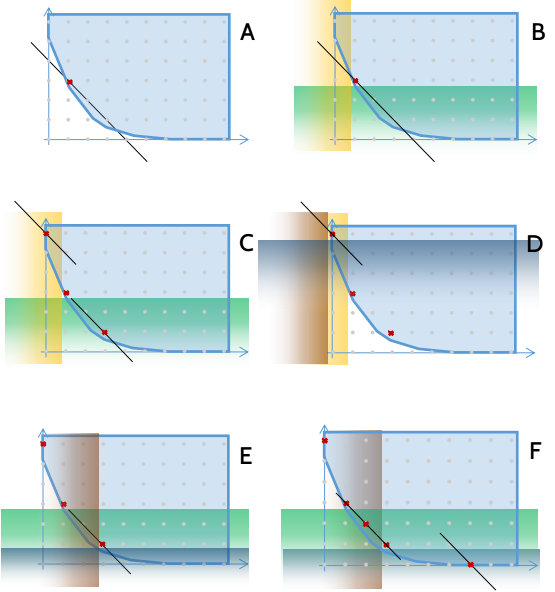
\includegraphics[scale=1]{example.png}
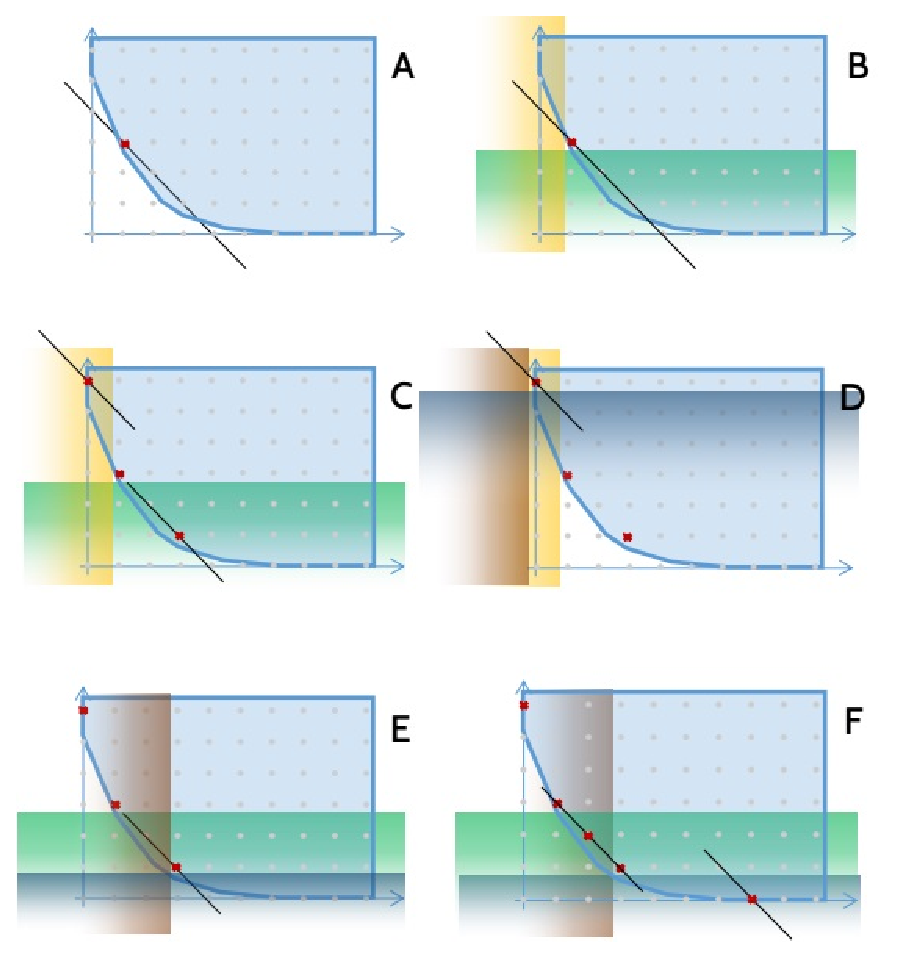
\includegraphics[scale=1]{example.eps}
\end{figure}







\subsection{Convergence Analysis}\label{sec:conv}
The Frontier Partitioner Algorithm requires that $\gamma>0$ for all objective functions $y_i(x)$, $i=1,2$ in~\eqref{BOIP}\red{, otherwise as shown in Proposition \ref{prop:gamma0} the problem is trivial and can be solved by applying any scalarization techniques assuring to find a Pareto point (e.g. the ones in Section \ref{sec:scal}).}

\begin{assumption}[Positive gap value]\label{ass:gamma}
The functions $y_i:\R^n\rightarrow \R$ in Problem~\eqref{BOIP} satisfy $\gamma_i>0$, for $i=1,2$.
\end{assumption}
As a first step we prove that the cuts used in Algorithm~\ref{fig:FPA} induce a partition of the decision space.

\begin{proposition}\label{prop:part}
Let assumption \ref{ass:gamma} holds.
 Then $\mathcal{X}^k_1\,\cap \,\mathcal{X}^k_2 = \emptyset$ for all $k$ in Algorithm~\ref{fig:FPA}.
\end{proposition}
\begin{proof}
 Let $\hat x^k\in \mathcal{X}^k\cap \Z^n$ be an efficient point for~\eqref{BOIP} corresponding to the non-dominated value $\hat y^k$. Assume by contradiction that $ \X^{k}_1 \cap \X^{k}_2 \neq \emptyset$.
 Then $x \in \X^{k}_1 \cap \X^{k}_2$ exists and it satisfies $y_i(x) <y_i(\hat{x}_k)$, for $i=1,2$ as $\epsilon_i>0$ by assumption. This contradicts the fact that
 $\hat x^k$ is an efficient solution for~\eqref{BOIP}.
\end{proof}



\begin{proposition}\label{prop:Yfinite}
Let assumptions \ref{ass:boip} and \ref{ass:gamma} hold.
Then, the Pareto frontier $\mathcal{Y}_N$ is a finite set.
\end{proposition}
\begin{proof}
Under Assumption \ref{ass:boip} there exist
$$\hat x^{i}\in \arg\min_{\mathcal{X}\cap \Z^n} y_i(x),\  i=1,2.$$
Hence there exist the values
$$M_1= y_1(\hat x^{2})\qquad M_2= y_2(\hat x^{1})$$
and
the Pareto frontier $\mathcal{Y}_N\subseteq \mathcal{Y}$ is contained in the box
$$[y_1^{id}, M_1]\times [y_2^{id}, M_2]$$
and hence it is bounded.
Each objective function $y_i$ can attain at most $\frac{M_i - y_i^{id}}{\gamma_i}$ distinct values, so that the cardinality of the Pareto frontier,
obtained as the combination of the two, is finite and at most
\[\frac{(M_1 - y_1^{id})(M_2 - y_2^{id})}{\gamma_1 \gamma_2}\]
\end{proof}
\red{AGGIUSTATO PER AVERE CORRISPONDENZA PADRI FIGLI A QUALSIASI LIVELLO:
\begin{proposition}\label{prop:nondom}
 Let $\hat y\in \mathcal{Y}_N^k$ be a non-dominated point of~\eqref{BOIP}$^k$.
 Then, problem
\begin{equation}\label{INLP}
\begin{array}{l l}
    \min & y(x)\\
    \textnormal{ s.t. }& x\in \mathcal{X}^k \cap \{ y_i(x)\leq \hat y_i - \epsilon_i\}\\
    & x\in\Z^n
  \end{array}
 \end{equation}
 with $i=1$ or $i= 2$ is either infeasible or its solutions are efficient for~\eqref{BOIP}$^k$.
 \end{proposition}
\begin{proof}
If problem (INLP)$^k$ is infeasible there is nothing to prove.
Let $i=1$ and let $\bar x$ be an efficient solution for (INLP)$^k$
(case $i=2$ can be proven identically).
By contradiction, assume that $\bar x$ is not efficient for~\eqref{BOIP}$^k$.
Then, $\tilde x\in \mathcal{X}^k \cap \Z^n$ exists
such that  $y_i(\tilde x)\leq y_i(\bar x)$, for $i=1,2$  and  $y(\tilde x)\neq y(\bar x)$.
In particular, we have that
\[y_1(\tilde x)\leq  y_1(\bar x) \leq  \hat y_1 - \epsilon_1\]
so that $\tilde x$ is feasible for (INLP)$^k$.
Since $y(\tilde x)\neq y(\bar x)$, we necessarily have that either $y_1(\tilde x)< y_1(\bar x)$ or $y_2(\tilde x)< y_2(\bar x)$,
contradicting the fact that $\bar x$ is efficient for (INLP)$^k$.
\end{proof}
}
\red{
\begin{proposition}\label{prop:frontierasottoproblema}
 In the FPA algorithm, for each $t$ and for each $(BOIP)^k \in \cal L$ then $(INLP)^k$ is either infeasible or its solutions are efficient for \eqref{BOIP}.
\end{proposition}
\begin{proof}
For a certain value of $t$ we have a set $\cal L$ associated to a branching tree. Considering subproblem $k \in \cal L$, if $k=0$ then the statement holds trivially because we are in the root node, otherwise we apply by induction proposition \ref{prop:nondom}.  In fact proposition \ref{INLP} states that given a subproblem, then its children if are feasible can return only efficient points which are efficient also for the father. By induction these points are efficient also for the subproblem generating the father itself, going backward in the tree until we reach the root node.  
\end{proof}
}

\red{
\begin{proposition}\label{prop:properties}
Suppose to have an efficient point $x_k \in {\cal X}^k$ associated to the subproblem $(BOIP)^k$, with associated set ${\cal X}^k$ and children $(BOIP)^{k'}$ and $(BOIP)^{k''}$. Let's call ${\cal X}^{k'} = {\cal X}^k \cup \left\{ x \in \setRn : y_1 (x) \le y_1(x^k) - \eps_1 \right\} $ and  ${\cal X}^{k''} = {\cal X}^k \cup \left\{ x \in \setRn : y_2 (x) \le y_2(x^k) - \eps_1 \right\} $, where $\eps_i \in \left( 0, \gamma_i \right] $, with $\gamma_i$ respecting definition \ref{def:gammah} for $i = 1,2$. Called ${\cal Y}^k_N$ the Pareto frontier of $(BOIP)^k$, the following property holds
$$
 {\cal Y}^k_N \smallsetminus \left\{ y(x^k) \right\} = {\cal Y}^{k'} \cup {\cal Y}^{k''}
$$
\end{proposition}
}


\begin{proof}
\red{Let us call $y\left( {\cal X}^k \cap \setZn \right)$ the projection of the set  ${\cal X}^k \cap \setZn$ in the objective space. }

\red{We first prove
\begin{equation}\label{inclusion}
    {\cal Y}^k_N \smallsetminus \left\{ y(x^k) \right\} \subseteq {\cal Y}^{k'} \cup {\cal Y}^{k''}
\end{equation}
Under definition \ref{def:dominated} and under the hypothesis for $\eps_1$ and $\eps_2$, if a different Pareto point exists and it is associated to an efficient solution in ${\cal X}^k \cap \setZn$ then one of the following two condition have to be satisfied
$$ y_1 (x) \le y_1(x^k) - \eps_1  \text{ or } y_2 (x) \le y_1(x^k) - \eps_2 $$
In other words if exists another Pareto Point $\hat{y} \neq y(x^k)$, $\hat{y} \in {\cal Y}^k$, then one of the two following holds
$$\hat{y} \in  y\left( {\cal X}^{k'} \cap \setZn \right) \text{ or } \hat{y} \in  y\left( {\cal X}^{k''} \cap \setZn \right) $$
This implies the following
\begin{equation}\label{coverproperty}
   {\cal Y}^k_N \smallsetminus \left\{ y(x^k) \right\} \subseteq  y\left( {\cal X}^{k'} \cap \setZn \right) \cup y\left( {\cal X}^{k''} \cap \setZn \right) 
\end{equation}
If \eqref{coverproperty} holds then suppose by contradiction that a Pareto point $\hat{y} \in {\cal Y}^k_N \smallsetminus \left\{ y(x^k) \right\}$ exists such that $\exists \tilde{y} \in {\cal Y}^{k'} \cup {\cal Y}^{k''}$ such that $\tilde{y} \le \hat{y}$, $ \tilde{y} \neq \hat{y}$. But this implies that an efficient point $\tilde{x}$ exists such that it is feasible for $(BOIP)^{k'}$ or $(BOIP)^{k''}$ and $\tilde{y} = y (\tilde{x})$. Since ${\cal X}^{k'} \subseteq {\cal X}$ and ${\cal X}^{k''} \subseteq {\cal X}$ this is in contradiction with the fact that $\hat{y}$ is Pareto. This shows that \eqref{inclusion} holds.
}


\red{
On the other hand we want to show $\ds {\cal Y}^k_N \smallsetminus \left\{ y(x^k) \right\} \subseteq  y\left( {\cal X}^{k'} \cap \setZn \right) \cup y\left( {\cal X}^{k''} \cap \setZn \right)$.%is implied combining proposition \ref{prop:nondom} and the fact that
We start by showing $\ds {\cal Y}^{k'} \cap {\cal Y}^{k''} = \emptyset$, by contradiction if a point $\hat{y} = y(\hat{x}) \in {\cal Y}^{k'} \cap {\cal Y}^{k''} $ this implies $\hat{x} \in {\cal X}^{k'} \cap {\cal X}^{k''} \cap \setZn$ which is empty, otherwise $y(x^k)$ is not Pareto. Combining this result with proposition \ref{prop:nondom} the inclusion holds. 
}
\end{proof}

\red{
\begin{proposition}\label{prop:nest}
 Under the hypothesis of proposition \ref{prop:properties}, called ${\cal K} = \left\{  k : (BOIP)^k \right.$ has been processed returning a solution $\left. x^k \right\}$  the following holds
 $${\cal Y}_N =    \bigcup_{t : (BOIP)^t \in {\cal L}} {\cal Y}^k_N \cup \bigcup_{k \in {\cal K}} \left\{ y (x^k) \right\}$$
\end{proposition}
}

\red{
\begin{proof}
It arise by applying recursively \ref{prop:properties} to all the nodes in the branching tree which are non-empty. The leaf nodes are the subproblem in $\cal L$ and the inner non-empty nodes are the ones indexed by $\cal K$. The recursion stops at the root node where ${\cal Y}_N^{root} = {\cal Y}_N$.
\end{proof}
}



\begin{theorem}\label{theo: convergence}
Let assumptions \ref{ass:boip} and \ref{ass:gamma} hold.
 Algorithm~\ref{fig:FPA} returns the complete Pareto frontier $\mathcal{Y}_N$ of~\eqref{BOIP} after having addressed
$2|\mathcal{Y}_N|+1$ scalar objective integer programs.
\end{theorem}
\begin{proof}
When node $(BOIP)^k$ is addressed in Algorithm~\ref{fig:FPA}, the integer program $(INLP)^k$ is built
using  a correct
scalarization technique (see Section~\ref{sec:scal}).
Then, Problem $(INLP)^k$ is solved: if $(INLP)^k$ is infeasible, we conclude that $\X^k\cap \Z^n$ does not contain any efficient point and the node is pruned.
Otherwise, from\red{ Proposition~\ref{prop:frontierasottoproblema}}, we have that its solutions are efficient points for (BOIP), giving us a non-dominated point $\hat y^k$.
By Proposition \ref{prop:part} and Remark~\ref{rem:const}, the non-dominated point $\hat y^k\in \mathcal{Y}_N$ cannot be detected again by
addressing any subsequent node in the branching tree.
 %In fact, $y(x)\neq \hat y^k$, for any $x\in \X^k_1\cap \Z^n$, or $x\in \X^k_2\cap \Z^n$ (see)
%and $\X^k_i\cap \Z^n$ is strictly contained in $\X^{k}\cap \Z^n$ for $i=1,2$.

\red{The procedure go on until all the Pareto points are found. Under the hypothesis of the theorem Proposition \ref{prop:nest} holds and it assures that at each iteration we are covering all the remaining Pareto points.}
Summarizing, whenever a node is addressed and an integer program is solved, either we get a new non-dominated point or we detect infeasibility
and we prune the node.
Therefore, since Algorithm~\ref{fig:FPA} produces exactly two children for each non-dominated point of~\eqref{BOIP},
we have that the branching tree has exactly  $2|\mathcal{Y}_N|+1$ nodes (including the root node) so that exactly  $2|\mathcal{Y}_N|+1$  integer programs will be addressed before finding the complete Pareto frontier.
\end{proof}

The total number of iterations of \texttt{FPA} is $O(|\mathcal{Y}_N|)$ that is in fact the order of complexity of any algorithm
 that aims to identify all
$|\mathcal{Y}_N|$ non-dominated points by solving a sequence of subproblems, as it must solve at least
$|\mathcal{Y}_N|$ subproblems.

We observe that, for the special case of linear BOIPs, a criterion space search algorithm
that solves $2|\mathcal{Y}_N|-1$ integer programs has been defined in~\cite{ralphs2006improved}.
So, in the linear case, this algorithm based on the augmented weighted Tchebycheff method, has a slightly better bound than our.
However, it is not straightforward how to extend the augmented weighted Tchebycheff method to tackle nonlinear BOIPs.

%The bound in the number of integer programs to be solved given in Theorem~\ref{theo: convergence} is actually worst then the one found in~\cite{ralphs2006improved},
%where an algorithm for biobjective linear integer programming was proposed and the number of integer programs to be solved is bounded by $2|\mathcal{Y}_N|-1$.
%\todo[inline]{Can we also use a smart ordering?}
\subsection{$\gamma$ and oracles}
In this section we present classes of functions that easily satisfy the Assumptions~\ref{ass:oracle} and~\ref{ass:gamma}.


As a first step we look for sufficient conditions to have $\gamma>0$ and computable whenever $f(x)\neq f(z)$ for all $x,z \in \X\cap \Z^n$ (Assumption~\ref{ass:gamma}).
\begin{proposition}\label{prop:suffcond}
Assume that $f:\Z^n\rightarrow \Z$. Then we get that $\gamma = 1$.
\end{proposition}
\begin{proof}
Since the image of $\mathcal{X}\cap \Z^n$ under $f$ is a subset of $\Z$, we have that $ |f(x) - f(z)| \ge 1$, for all $x,z \in \X\cap \Z^n$ such that $f(x) \neq f(z)$.
\end{proof}

\begin{remark}As a matter of example of functions satisfying the condition in Proposition~\ref{prop:suffcond} we have all the polynomials with integer coefficients and in particular  $f(x) = c^\top x$ with  $c\in \Z^n$ and $f(x) = x^\top Q x + c^\top x$ with $Q \in \Z^{n\times n}$ and $c \in \Z^n$.
\end{remark}
We look now for larger classes of functions for which $\gamma >0$: we focus on functions defined on rational domains.
\begin{proposition}\label{prop:condquad}
Let $f(x) = x^\top Q x + c^\top x $.
Assume that $Q \in \Q^{n\times n}$ and $c \in \Q^n$, then $r \in \N$, $r\neq 0$ exists so that $\gamma = \frac{1}{r}$.
\end{proposition}
\begin{proof}
Since $Q \in \Q^{n\times n}$ and $c \in \Q^n$ then $r \in \N$, $r\neq 0$ exists such that $rQ \in \Z^{n\times n}$ and $rc \in \Z^n$.
The function $g(x) = x^\top (rQ) x + (rc)^\top x = r f(x)$ satisfies the assumption of Proposition~\ref{prop:suffcond}, therefore we can write
\[
| g(x) - g(z) | \ge 1, \ \ \forall \ x,z \in \X \cap \Z^n: g(x) \neq g(z) \\
\]
or, equivalently,
\[
| f(x) - f(z) | \ge \frac{1}{r}, \ \ \forall \ x,z \in \X\cap \Z^n : f(x) \neq f(z).
\]
\end{proof}

Note that $r$ is easily calculable as the least common multiple of the denominators of the rational coefficients.

\red{
\begin{proposition}
 Let $f(x): \setZn \rightarrow \setR$ be a polynomial with rational coefficients, with at least one different from zero. The $r \in \setN$, $r \neq 0$ exists so that $\gamma = \frac{1}{r}$.
\end{proposition}
\begin{proof}
We can easily write $ f(x) = \sum_{k = 0}^{s} \alpha_k q_k(x)$, where $q_k(x) = \prod_{i=1}^n x_i^{m_{i k}}$ and $m_{i k } \in \setN$, for $k=0,\dots,s$, $i = 1, \dots, n$. Since the entries are integers then $q_k(x) \in \setZ$, for $k = 0,dots, s$ and for all $x \in \setZn$. We know that exist $r \in \setN$, $r \neq 0$ such that $r \alpha_k \in \setZ$, $k=0,\dots,s$. The proof is now equal to the one in Proposition \ref{prop:condquad}, since we are acknowledging $g(x) = r f(x) $ satisfies the assumption of Proposition \ref{prop:suffcond}
\end{proof}
}
\todo[inline]{\st{Polynomials in $n$ variables seem to satisfy the condition. Check how to write polynomials and the assertion}}
\begin{remark}
Of course Proposition~\ref{prop:condquad}  holds when $Q$ is the zero matrix, i.e. when $f(x)$ is a rational linear function: $f(x) = c^\top x $,  $c \in \Q^n$.
\end{remark}

\begin{proposition}\label{prop:condquad}
Let $f(x) =\|A x+ b\|_2 $ and assume that $$\bar v=\max_{x \in \X\cap \Z^n} \|A x+ b\|^2_2 \in \R_+\setminus \{\infty\}.$$
Assume that $A \in \Z^{m\times n}$ and $b \in \Z^n$, then  $\gamma = \sqrt{\bar v+1}-\sqrt{\bar v}$.
\end{proposition}
\begin{proof}
%Let $x,z \in \X\cap \Z^n$ such that $f(x) \neq f(z)$, and $v=Ax+b$, $w=Az+b$ so that $v\neq w$.
Since $A \in \Z^{m\times n}$ and $b \in \Z^n$
we have that $(Ax+b)\in \Z^m$
for all $x \in \X\cap \Z^n$.
Therefore for all $x,z \in \X\cap \Z^n$ such that $f(x) \neq f(z)$ we get
\[
| f(x) - f(z) | = \left |\|A x+ b\|_2 -\|A z+ b\|_2\right|\ge
\left |\|v\|_2 -\|w\|_2\right|
\]
with $v, w\in \Z^m$ such that $v\neq w$ and they differ exactly for one component, which is the least difference possible.
 We can assume  w.l.o.g. that $ v_i= w_i$ for all $i\neq j$ and $ w_j= v_j+1$ and we finally get

\[
| f(x) - f(z) | \ge  \left |\sqrt{\sum_{i=1}^m v_i^2} -\sqrt{\sum_{i=1}^m v_i^2+2v_j+1}\right|\ge \sqrt{\|v\|^2+1}-\sqrt{\|v\|^2}.
\]

Let $g(x)=\|A x+ b\|^2_2$, the function $\sqrt{g+1}-\sqrt{g}$ is monotonically decreasing hence it attains its minimum value at its upper bound $\bar v$ and
\[
| f(x) - f(z) | \ge   \sqrt{\bar v+1}-\sqrt{\bar v}.
\]
\end{proof}

\red{
\st{In order to satisfy Assumption}~\ref{ass:oracle}\st{, we need an oracle able to address Problem $(INLP)^k$: }
\begin{equation*}
    \min_{\mathcal{S}\cap \Z^n} y_1(x) + y_2(x) DELETED
 \end{equation*}
\st{where $\mathcal{S}$ is obtained intersecting the original decision space $\mathcal{X}$ with a finite number of cuts
of the type $\{x\in \R^n \,:\,y_i(x)\leq \alpha\}$, $i=1,2$, $\alpha\in \R$.}
\st{In particular, we restrict ourselves to convex objectives $y_i(x)$, so that $\mathcal{S}\subseteq \R^n$ is convex.}}

In Table \ref{tab:classes}, we report some classes of objective functions that can be considered when using integer programming solvers
such as CPLEX~\cite{cplex-url}, Gurobi~\cite{gurobi}, SCIP~\cite{GleixnerEiflerGallyetal.2017}, Couenne \cite{} or Bonmin~\cite{bonami2008algorithmic},
in order to deal with problem $(INLP)^k$.
In particular,
\begin{itemize}
 \item if both $y_i(x)$ $i=1,2$ are linear, then $(INLP)^k$ is an Integer Linear Program (ILP);
 \item if one $y_i(x)$ is written as $\|Ax + b\|_2$, then $(INLP)^k$ is an Integer Second Order Cone Program (ISOCP);
 \item if one $y_i(x)$ is convex quadratic, then $(INLP)^k$ is a Quadratically Constrained Quadratic Integer Program (QCQIP);
 \item if one $y_i(x)$ is general convex, then $(INLP)^k$ is a Convex Integer Program (CIP).
\end{itemize}

\begin{table}[h!]
\caption{Classes of functions that satisfy Assumptions~\ref{ass:oracle} and~\ref{ass:gamma}. In the table we denote with $r$ the least
common multiple of the denominators of the rational coefficients.}\label{tab:classes}
\begin{tabular}{||l| c| c||}
\hline\hline
$y_i(x)=$ & $\gamma$ & oracle\\
\hline\hline
& & \\[-1.5ex]
$  c^\top x$ with $c\in \Z^n$ & $1$ & \emph{ILP}\\[1.5ex]
$  c^\top x$ with $c\in \Q^n$ & $\frac 1 r$ & \emph{ILP}\\[1.5ex]
$  \|Ax +b\|_2$ with $A\in \Z^{n\times m}$, $b\in \Z^m$  & $\sqrt{\bar v+1}-\sqrt{\bar v}$ & \emph{ISOCP}\\[1.5ex]
$  x^\top Q x + c^\top x$ with $Q\succeq 0$, $Q\in \Z^{n\times n}$, $c\in \Z^n$  & $1$ & \emph{QCQIP}\\[1.5ex]
$  x^\top Q x + c^\top x$ with $Q\succeq 0$, $Q\in \Q^{n\times n}$, $c\in \Q^n$  & $\frac 1 r$ & \emph{QCQIP}\\[1.5ex]
$:\Z^n\rightarrow \Z$, convex & $1$& \emph{CIP}\\[1.0ex]
\hline\hline
\end{tabular}
\end{table}


%\subsection{Inducing linear cuts}
\subsection{Circumventing/Encompassing/Bypassing nonlinear cuts}
We introduced the Frontier Partitioner Algorithm as a branch and cut algorithm: new nodes are built imposing cuts
to the feasible set in the decision space (see Step~\ref{step:newnodes} in Algorithm~\ref{fig:FPA}).
More specifically, at a generic node $k$, the set $\mathcal{X}^k \cap \Z^n$ is intersected with the following set:
\begin{equation}\label{eq:cut}
C =\{x\in \R^n\,:\, y_i(x)\leq \hat y^k_i - \epsilon_i \},
\end{equation}
being $i=1$ or $i=2$ and $\hat y^k$ the non-dominated point found at node $k$.
When $y_i(x)$ is convex nonlinear we are introducing a nonlinear cut, as
the set in~\eqref{eq:cut} is defined according to a nonlinear inequality.
However, we do not necessarily need to add nonlinear inequalities:
for our purposes, it would suffice to define a valid formulation for the integer
set $\{x\in~\Z^n\,:\,~y_i(x)\leq\hat y_i - \epsilon_i\}$,
or, in other words, it would suffice to find a matrix $A\in \R^{m\times n}$ and a vector $b\in \R^m$ such that
\begin{equation}\label{eq:lincuts}
\{x\in \Z^n\,:\, A x\leq b\} =  \{x\in \Z^n\,:\, y_i(x)\leq \hat y_i - \epsilon_i \}.
\end{equation}
Such a valid formulation can be obtained, at least theoretically, when $\mathcal{X}$ is compact and we deal with convex inequalities:
in~\cite{dadush:2011, dadush:2014} it is shown that
the Chv\'atal--Gomory closure of a compact convex set is a rational polyhedron.
However, from a practical point of view, it is not yet clear how to easily generate a valid formulation.

It is the purpose of this section to investigate on the use of linear inequalities within \texttt{FPA}.

Under the assumption that $y_i:\R^n \rightarrow \R$ is convex and continuously differentiable, we have that
 \[\nabla y_i(\hat x^k)^\top (\hat x^k - x) \geq y_i(\hat x^k) - y_i(x) \geq \epsilon_i.\]
Therefore, we can think of defining $\mathcal{X}^{k}_i$ intersecting $\mathcal{X}^k$ with the
halfspace \[\{x\in \R^n\,:\, \nabla y_i(\hat x^k)^\top (\hat x^k - x)\geq \epsilon_i\}.\]
The resulting \texttt{FPA}, may eventually not terminate with the entire Pareto frontier, as we are not guaranteed
of cutting the current non-dominated point.
On the one hand, we loose the exactness of the method, but we have the advantage of dealing with linear constraints.


For the specific class of problems where the objectives are strictly convex quadratic forms,
we can prove the following result:
\begin{proposition}\label{prop:lincuts}
 Let $y_i(x) = x^\top Q x$, with $Q\succ 0$.
 Then
   \[C\cap \Z^n \subseteq C^1\cap C^\infty\]
  where
    \[C^1 = \Big\{x\in \Z^n\,:\, \|Q^{1/2} x\|_1 \leq \frac 1  {\sqrt{n}}\sqrt{\hat y_i - \epsilon_i} \Big\} \]
and
   \[C^\infty = \Big\{x\in \Z^n\,:\, \|Q^{1/2} x\|_\infty \leq \sqrt{\hat y_i - \epsilon_i} \Big\} \]

\end{proposition}

\begin{proof}
We have that
 \begin{equation*}\label{eq:2norm}
 \begin{array}{l l}
  \{x\in \Z^n\,:\, y_i(x)\leq \hat y_i - \epsilon_i \} &= \{x\in \Z^n\,:\, x^\top Q x \leq \hat y_i - \epsilon_i \} \\ [1.3ex]
  &= \{x\in \Z^n\,:\, \|Q^{1/2} x\|_2^2 \leq \hat y_i - \epsilon_i \} \\[1.3ex]
  &= \{x\in \Z^n\,:\, \|Q^{1/2} x\|_2 \leq \sqrt{\hat y_i - \epsilon_i} \}=C\cap \Z^n
 \end{array}
\end{equation*}
Using the relations between   norms  $ {\sqrt{n}}\|x\|_2 \leq  \|x\|_1$ and $ \|x\|_2 \geq  \|x\|_\infty$ we have that
$$\begin{array}{l l}
C\cap \Z^n
  &\subseteq C^1=\{x\in \Z^n\,:\, \|Q^{1/2} x\|_1 \leq \frac 1  {\sqrt{n}} \sqrt{\hat y_i - \epsilon_i}\}\\[1.3em]
C\cap \Z^n
  &\subseteq C^\infty=\{x\in \Z^n\,:\, \|Q^{1/2} x\|_\infty \leq  \sqrt{\hat y_i - \epsilon_i}\}
\end{array}
$$
hence we get the result.\end{proof}

%\begin{proposition}\label{prop:lincuts}
% Let $y_i(x) = x^\top Q x$, with $Q\succ 0$.
% Then
%   \[C\cap \Z^n \supseteq C_{lin}\]
%  where
%   \[C_{lin} = \Big\{x\in \Z^n\,:\, \|Q^{1/2} x\|_1 \leq \sqrt{\hat y_i - \epsilon_i} \Big\} \]
% % \[S_{lin} = \Big\{x\in \Z^n\,:\, \|Q^{1/2} x\|_1 \leq \sqrt{\hat y_i - \epsilon_i} \;,\;  \|Q^{1/2} x\|_\infty \leq \frac{1}{\sqrt n}\sqrt{\hat y_i - \epsilon_i} \Big\} \]
%\end{proposition}
%\begin{proof}
%We have that
% \begin{equation*}\label{eq:2norm}
% \begin{array}{l l}
%  \{x\in \Z^n\,:\, y_i(x)\leq \hat y_i - \epsilon_i \} &= \{x\in \Z^n\,:\, x^\top Q x \leq \hat y_i - \epsilon_i \} \\ [1.3ex]
%  &= \{x\in \Z^n\,:\, \|Q^{1/2} x\|_2^2 \leq \hat y_i - \epsilon_i \} \\[1.3ex]
%  &= \{x\in \Z^n\,:\, \|Q^{1/2} x\|_2 \leq \sqrt{\hat y_i - \epsilon_i} \}\\[1.3ex]
%  &\supseteq \{x\in \Z^n\,:\, \|Q^{1/2} x\|_1 \leq \sqrt{\hat y_i - \epsilon_i}\}
% \end{array}
%\end{equation*}
%where the last inclusion follows from the relations between the Euclidean and the Manhattan norm: $\|x\|_2 \leq \|x\|_1$.
%\end{proof}
%\todo[inline]{Purtroppo esiste un controesempio (imbecille): $x^0\in \Z^2$, $x^0 = (2,3)^\top$ $\|x^0\|_1 =5>4$, mentre $\|x^0\|_2=\sqrt{13}<4$}
Note that both $C^1$, $C^\infty$ are defined by $2n$ linear inequalities.
Hence in the specific case of problems with strictly convex quadratic forms as objective,
one can think of generating $(BOIP)^k$ using these $4n$ linear inequalities.
Again, the resulting \texttt{FPA} will be a heuristic approach, as we are not guaranteed
of cutting the non-dominated points found so far. However, we have the advantage of dealing with a quadratic integer programming
problem that can be solved quite efficiently with respect
to quadratically constrained quadratic integer programming instances (see, e.g.,~\cite{buchheim:2016}).

%\todo[inline]{General convex quadratic case}



\section{Numerical results}\label{sec:numres}
To test the performance of our algorithm~\texttt{FPA}, we considered biobjective integer linear instances (see Section~\ref{sec:explin}) and
biobjective integer quadratic instances (see Section~\ref{sec:expquad}).
Algorithm~\texttt{FPA} is implemented in Java and use \texttt{CPLEX 12.6} \todo{(??)} as integer programming solver.
All our experiments were carried out on
\todo[inline]{(Intel Xeon processors running
at 2.60~GHz...).}
All running times were measured in CPU seconds.
All tables presented in this section include the following data for the
comparison...


Problem $(INLP)^k$ is built by using the Goal programming method with $q = 1$ (see Section~\ref{sec:scal} and in particular Remark~\ref{rem:q1}).
This means that at every node of our branch and cut we address
the following integer program
\begin{equation}
 \min_{x\in \mathcal{\X}_i^k\cap \Z^n} y_1(x) + y_2(x),
\end{equation}
for some $i=1,2$.

\todo[inline]{Confronto da diverse tecniche di scalarizzazione: noi contro di noi. Scelta di quella che performa meglio come tempi e confronto con altri}

\subsection{Numerical experiments on linear instances}\label{sec:explin}
In this section, we present a numerical comparison of algorithm~\texttt{FPA} with the
balanced box method proposed in~\cite{boland2015criterion}, that in the following is denoted as \texttt{BBM}.
\todo[inline]{description of the instances}
We considered in total $219$ biobjective integer linear instances:
$n1$ instances of the biobjective knapsack problem, $n2$ instances of the biobjective assignment problem and $n3$
instances of biobjective integer linear programming.
The instances considered have been used in~\cite{boland2015criterion} and are available on \url{htt:\\...}.


Besides the tables of average running times, we visualize our results comparing the performance of~\texttt{FPA} and~\texttt{BBM}
by performance profiles, as proposed in~\cite{DM2002}.
Given our set of solvers $\mathcal{S}$=\{\texttt{FPA},~\texttt{BBM}\} and a set of problems $\mathcal{P}$,
we compare the performance of  a solver $s \in \mathcal{S}$ on problem $p \in \mathcal{P}$
against the best performance obtained by any solver in $\mathcal{S}$
on the same problem. To this end, we define the performance ratio
$
%\[
r_{p,s} = t_{p,s}/\min\{t_{p,s^\prime}: s^\prime \in\mathcal{S}\},
%\]
$
where $t_{p,s}$ is the computational time, and we consider a cumulative distribution
function
\[
\rho_s(\tau) = |\{p\in \mathcal{P}:\; r_{p,s}\leq \tau \}| /|\mathcal{P}|.
\]
The performance profile for $s \in S$ is the plot of the function $\rho_s$.

% \begin{figure}[h!]
%   \begin{center}
%      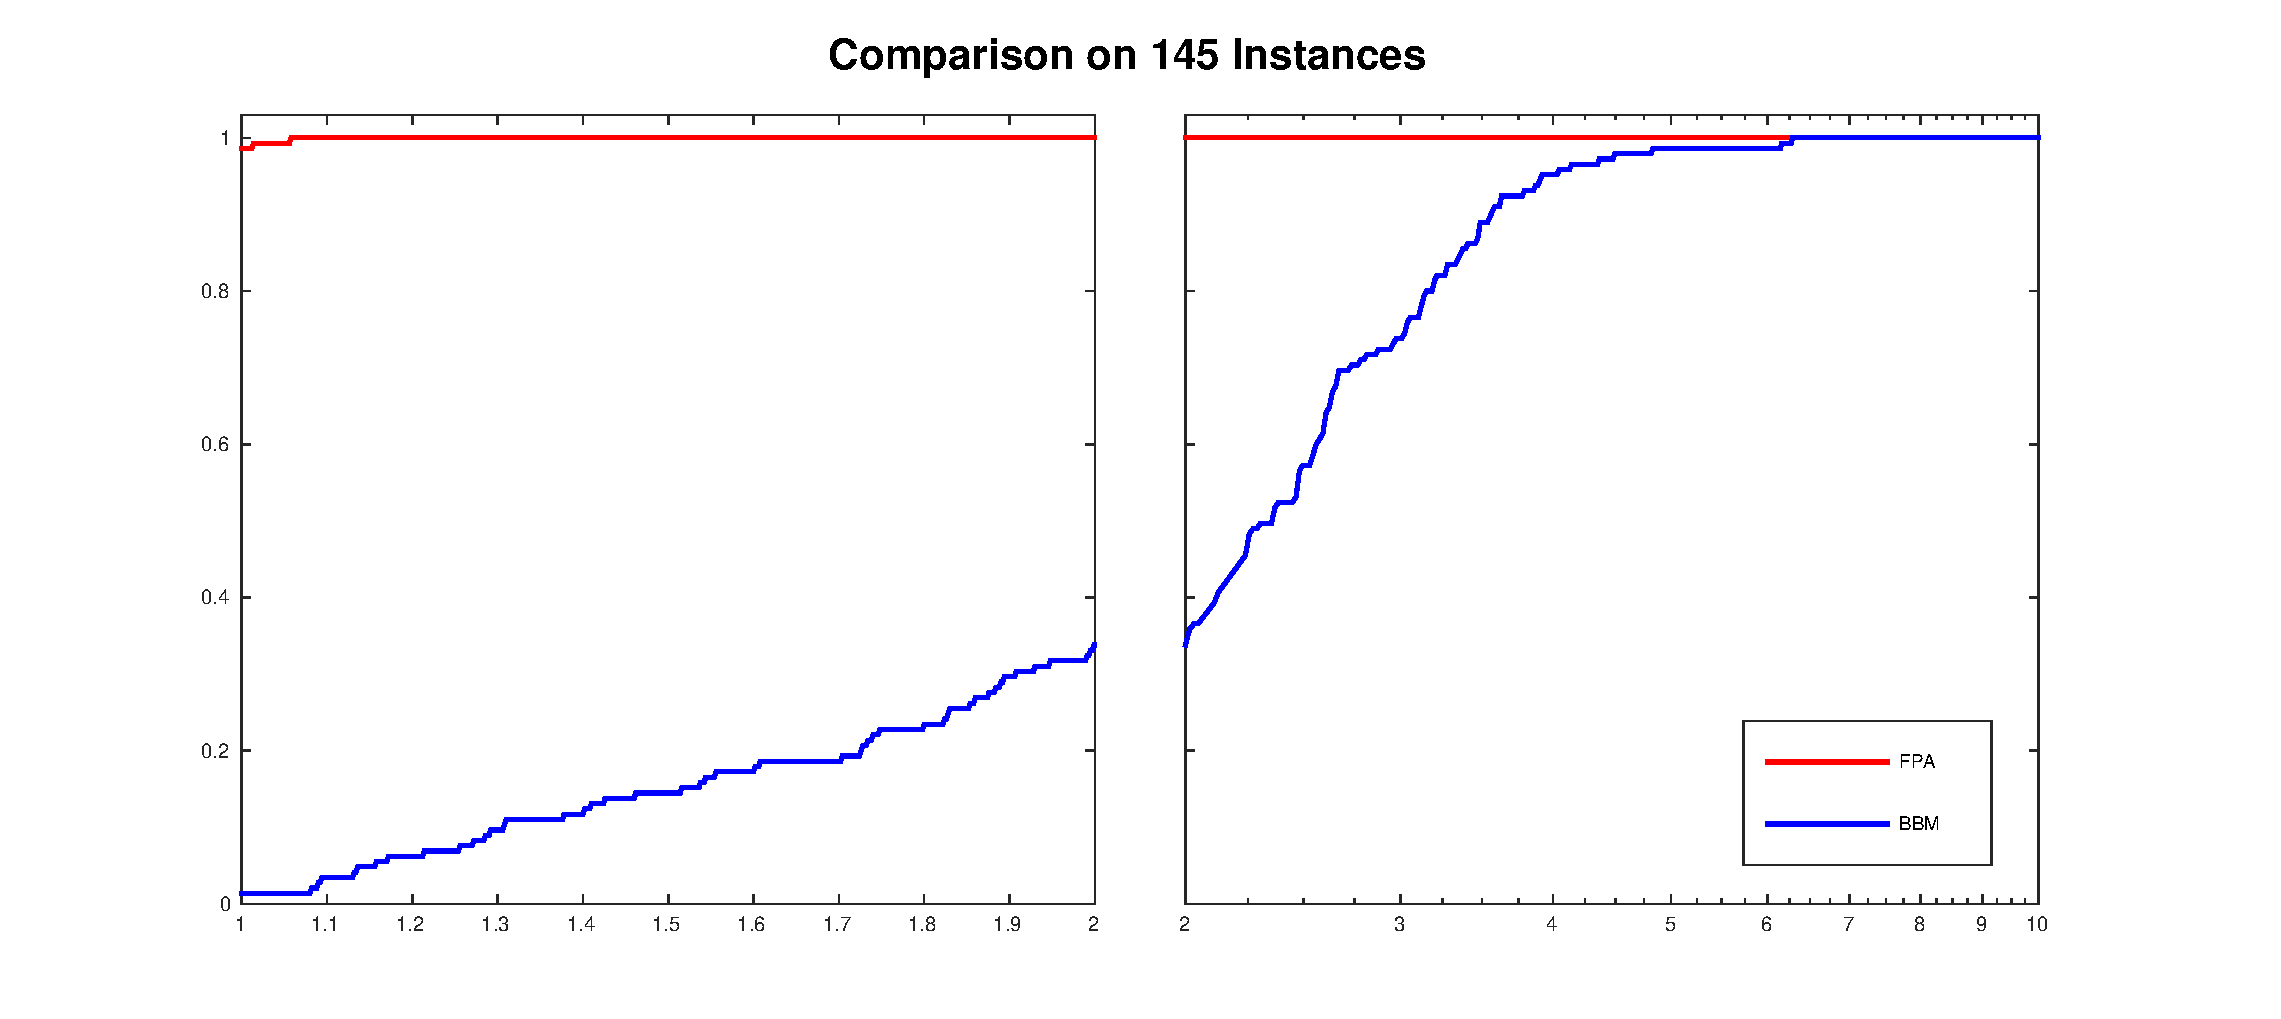
\includegraphics[clip, width=1.0\textwidth]{Figure/PerfProf.eps}\\
%     \caption{Performance Profiles - results with four threads.}
%     \label{fig:contour}
%   \end{center}
% \end{figure}

\subsubsection{Biobjective Knapsack Problem}\label{sec:num-kp}
Let $b\in \Z$ be the capacity of the knapsack, $a_i > 0, a_i\in \Z$ be the weight
and $c_{1i}, c_{2i}\in \Z$ be the profits of the
$i$-th object.
The biobjective Knapsack Problem can be modeled as follows:
\begin{equation*}\label{BOIKP}
\begin{array}{l l}
    \max & (c_{1}^\top x,\, c_2^\top x)\\[1.2ex]
    \textnormal{ s.t. }&  a^\top x \leq b\\[1.2ex]
    & x\in\{0,1\}^n.
  \end{array}
 \end{equation*}
In the instances considered we have $c_{ij}, a_j\in[1,1000]$, with $j=1,\ldots,n; \; i=1,2$ and $b = \big\lceil 0.5 \sum_{j=1}^n a_j \big\rceil$.
Note that the condition in Proposition~\ref{prop:suffcond} is satisfied, so that $\gamma=1$.
\todo[inline]{Table - results with one thread}
\todo[inline]{Performance profiles - results with one thread}

\subsubsection{Biobjective Assignment Problem}\label{sec:num-ap}
The biobjective assignment problem aims to obtain optimal
assignments between a set of agents $j\in \{1,\ldots, n\}$ and a set of tasks $k\in \{1,\ldots, n\}$, where each assignment
has non-negative costs $c_{1jk},\, c_{2jk}$.
\begin{equation*}\label{BOIAP}
\begin{array}{l l l}
    \min & (\sum_{j=1}^n\sum_{k=1}^n c_{1jk},& \sum_{j=1}^n\sum_{k=1}^n c_{2jk}\big)\\[1.2ex]
    \textnormal{ s.t. }&  \sum_{k=1}^n x_{jk} = 1 & j=1,\ldots,n\\[1.2ex]
    &  \sum_{j=1}^n x_{jk} = 1 & k=1,\ldots,n\\[1.2ex]
    & x_{ij}\in\{0,1\}, & i=1,\ldots,n;\, j=1,\ldots,n.
  \end{array}
 \end{equation*}
In the instances considered we have $c_i\in \Z^{n\times n}$ and $c_{ijk}\in [1,20]$,\, $i=1,2;\; j=1,\ldots,n;\; k=1,\ldots,n$.
Note that the condition in Proposition~\ref{prop:suffcond} is satisfied, so that $\gamma=1$.
\todo[inline]{Table - results with one thread}
\todo[inline]{Performance profiles - results with one thread}

\subsubsection{Biobjective Integer Linear Programming Problem}\label{sec:num-lp}
The generic biobjective integer linear programming problem is modeled as
\begin{equation*}\label{BOILP}
\begin{array}{l l}
    \min & (c_1^\top x,\, c_2^\top x)\\[1.2ex]
    \textnormal{ s.t. }&  A x \leq b\\[1.2ex]
    & x\in\Z^n.
  \end{array}
 \end{equation*}
In the instances considered we have $c_i\in \Z^n$, $i=1,2$;\; $A\in \Z^{m\times n}$ and $b\in \Z^m$.
In particular, $c_{ij}$ is generated in the ranges $[-100,-1]$ with probability $0.2$ and $[0,100]$ with probability $0.8$,
$j=1,\ldots,n$; $i=1,2$. The coefficients $a_{kl}$ are generated in the ranges $[-100,-1]$ with probability $0.1$,
$[1,100]$ with probability $0.8$ and $a_{kl}=0$ with probability $0.1$.
The right-hand side $b_k$ is generated randomly in the range $100$ and $\sum_{l=1}^n a_{kl}$.
Note that the condition in Proposition~\ref{prop:suffcond} is satisfied, so that $\gamma=1$.
\todo[inline]{Table - results with one thread}
\todo[inline]{Performance profiles - results with one thread}



\subsection{Parallelization}
It is nowadays common to use computers with multiple cores.
This gives the possibility of dividing computations over multiple threads
and consequently reducing the running times. Commercial integer programming solvers as
\texttt{CPLEX} are designed
to exploit the availability of multiple threads: in \texttt{CPLEX} users can choose the number
of threads to use, by properly setting the parameter \texttt{CPX\_PARAM\_THREADS}.
In~\cite{boland2015criterion}, the authors discuss the benefits of using multiple threads
and this motivated the following numerical experiment.
We set \texttt{CPX\_PARAM\_THREADS} to \todo{(??)} in both our implementation of
\texttt{FPA} and in the C++ implementation of \texttt{BBM}.
\todo[inline]{Table - results with $p$ threads}
\todo[inline]{Performance profiles - results with $p$ threads}


\subsection{Numerical experiments on quadratic instances}\label{sec:expquad}
The generic biobjective integer quadratic programming problem is modeled as
\begin{equation*}\label{BOIQP}
\begin{array}{l l}
    \min & (x^\top Q_1 x + c_1^\top x,\, x^\top Q_2 x + c_2^\top x)\\[1.2ex]
    \textnormal{ s.t. }&  A x \leq b\\[1.2ex]
    & x\in\Z^n.
  \end{array}
 \end{equation*}
In the instances considered we have $Q\succ 0$,  $Q_i\in \Z^{n\times n}$, $c_i\in \Z^n$, $i=1,2$;\; $A\in \Z^{m\times n}$ and $b\in \Z^m$.
In particular, $Q_{ij}$ and $c_{ij}$ is generated in the ranges $[-100,-1]$ with probability $0.2$ and $[0,100]$ with probability $0.8$,
$j=1,\ldots,n$; $i=1,2$. The coefficients $a_{kl}$ are generated in the ranges $[-100,-1]$ with probability $0.1$,
$[1,100]$ with probability $0.8$ and $a_{kl}=0$ with probability $0.1$.
The right-hand side $b_k$ is generated randomly in the range $100$ and $\sum_{l=1}^n a_{kl}$.
Note that the condition in Proposition~\ref{prop:suffcond} is satisfied, so that $\gamma=1$.

\todo[inline]{description of the instances}
\todo[inline]{Table - results with one thread}

% Let $y_i(x) = x^\top Q_ix + c_i^\top x$, with $Q_i\succeq 0 $, $Q_i\in \Q^{n\times n}$ and $c_i\in \Q^n$. We are under the assumptions
% of Proposition~\ref{prop:condquad} so that $\gamma_i>0$ exists and we can define $\epsilon_i\in (0,\gamma_i]$.
% In this case, Problem $(INLP)^k$ is formed by adding the quadratic constraints
% $y_i(x) \le y_i(\hat{x}) - \epsilon_i$, ending with a convex quadratic quadratically constrained integer programming problem.
% However, we adopt the strategy described in Remark~\ref{rem:linearcuts}, so that  we introduce the following linear constraints
% \[
%  \nabla y_i(\hat{x})^\top \left(\hat{x} - x \right) \ge \epsilon_i,
% \]
% and $(INLP)^k$ results in a quadratic integer programming problem that can be solved with a smaller computational effort (see, e.g.,~\cite{buchheim:2016}).
% \todo[inline]{The resulting \texttt{FPA} is a heuristic...}

\section{Conclusions}\label{sec:conc}

\section{Acknowledgments}
The authors acknowledge Prof. Hadi Charkhgard for having kindly provided the code of the balanced box method~\cite{boland2015criterion}.

%\bibliographystyle{plain}
\bibliographystyle{abbrv}
\bibliography{frontierAlg}
	
\end{document}
